%!TeX root=main.tex

\section{Definición de funciones de varias variables}

Las funciones en varias variables se pueden definir
de la misma manera que se hace para una variable,
pero añadiendo variables adicionales en la definición
de la función.
Por ejemplo para definir la función
$f(x,y) = \cos(x^2)+\sen(y^2)$
se escribirá lo siguiente.
\begin{maximai}
 f(x,y):= cos(x^2) + sin(y^2);
\end{maximai}
\begin{maximao}
 \operatorname{f}\left( x\operatorname{,}y\right)
 \operatorname{:=}
 \cos{\left( {{x}^{2}}\right) }+\sin{\left( {{y}^{2}}\right) }
\end{maximao}
De la misma manera se puede calcular el valor en un punto,
por ejemplo para calcular el valor $f(\pi, 2\pi)$ se escribirá
\maximain{f(\%pi, 2*\%pi)}.

A continuación mostramos la posibilidad de definir funciones
a trozos en varias variables, por ejemplo la función
\begin{equation*}
 g(x,y) =
 \left\{
  \begin{array}{cl}
   xy\frac{x^2-y^2}{x^2+y^2} & \text{ si } (x,y)\neq(0,0),\\
   0 & \text{ si } (x,y) = (0,0).\\
  \end{array}
  \right.
\end{equation*}

\begin{maximai}
 g(x,y):= if (x=0 and y=0) then 0 else x*y*(x^2-y^2)/(x^2+y^2)$
\end{maximai}
\begin{maximai}
 g(1,2);
\end{maximai}
\begin{maximao}
 -\frac{6}{5}
\end{maximao}


\section{Gráficas de funciones de dos variables}

A continuación veremos diferentes comandos
de Maxima
para realizar gráficas de funciones en dos
variables.

\subsection{Usando \texttt{wxplot3d}}

Para graficar una función $f$ de dos variables
en el rectángulo $[a,b]\times[c,d]$, se puede
usar el comando \texttt{wxplot3d} de la siguiente
manera.
\begin{center}
 \maximain{wxplot3d(f(x,y), [x, a, b], [y, c, d])}
\end{center}
Por ejemplo, a continuación representamos gráficamente
las funciones definidas previamente.
\begin{maximai}
 wxplot3d(f(x,y), [x, -1, 1], [y, -1, 1])$
\end{maximai}
\begin{maximat}
 \hfill
 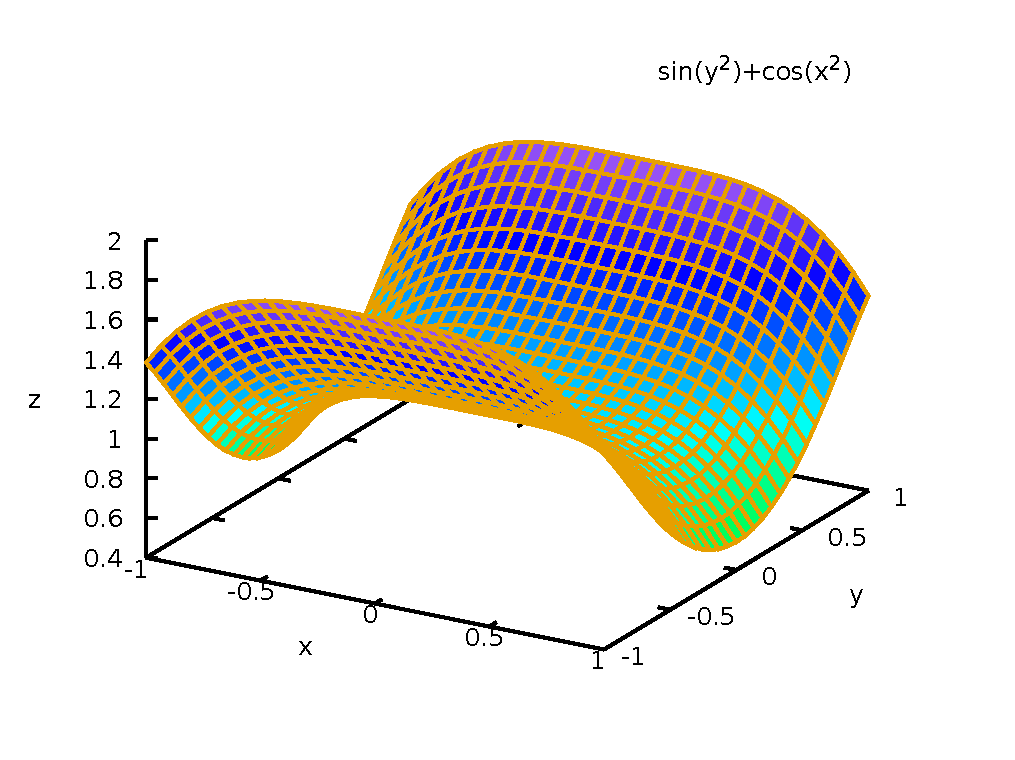
\includegraphics[width=.5\textwidth]{wxplot3d_f.pdf}
 \hfill
\end{maximat}

\begin{maximai}
 wxplot3d(g(x,y), [x, -1, 1], [y, -1, 1])$
\end{maximai}
\begin{maximat}
 \hfill
 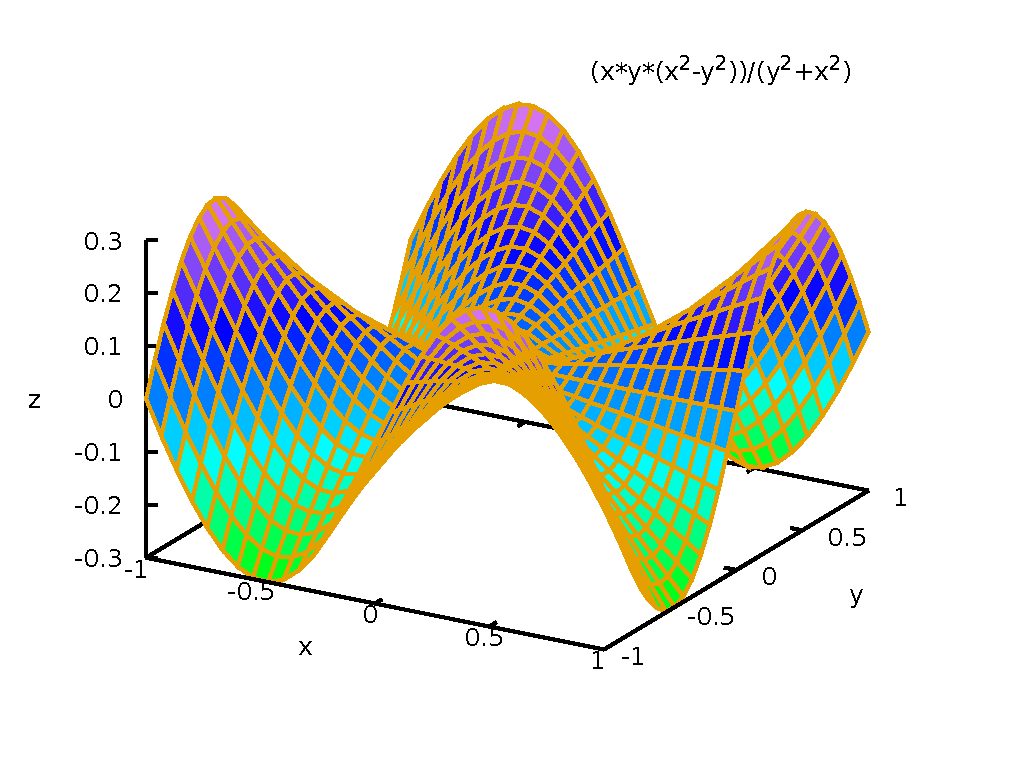
\includegraphics[width=.5\textwidth]{wxplot3d_g.pdf}
 \hfill
\end{maximat}

\subsection{Usando \texttt{wxcontour\_plot}}

Para realizar una representación de las curvas de nivel
de una función de dos variables usaremos el comando siguiente.
\begin{center}
 \maximain{wxcontour\_plot(f(x,y), [x,a,b], [y,c,d])}
\end{center}

A continuación mostramos las curvas de nivel de las funciones
definidas anteriormente.

\begin{maximai}
 wxcontour_plot(f(x,y), [x,-1,1], [y,-1,1])$
\end{maximai}
\begin{maximat}
 \hfill
 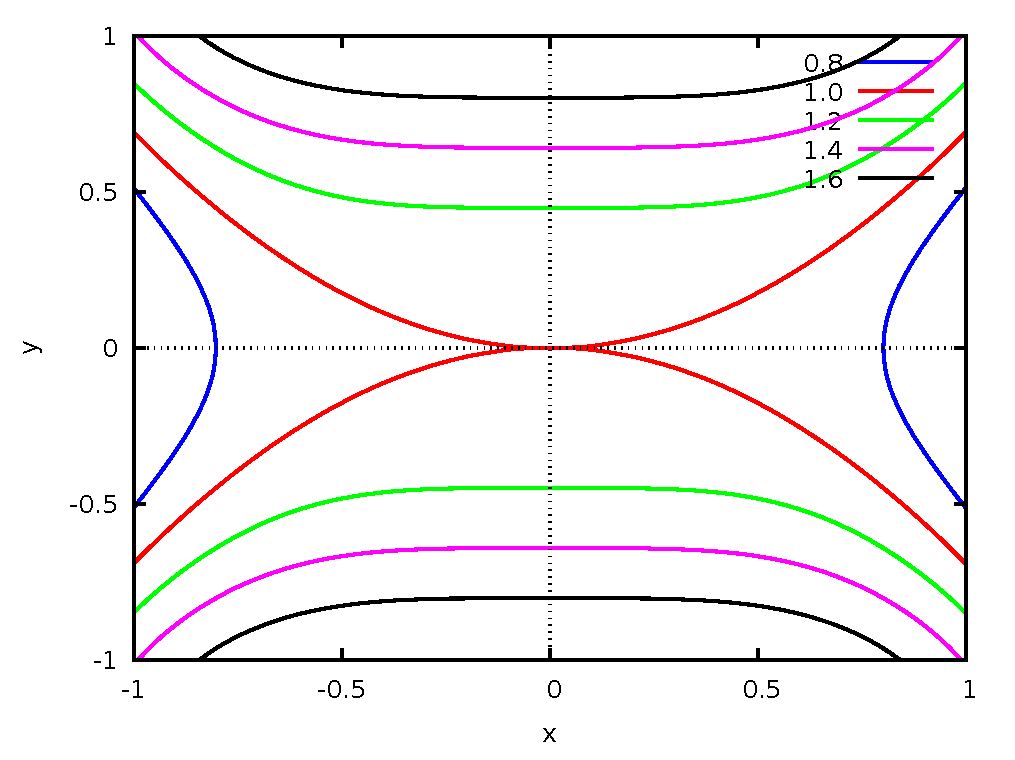
\includegraphics[width=.5\textwidth]{wxcontour_f.pdf}
 \hfill
\end{maximat}
\begin{maximai}
 wxcontour_plot(g(x,y), [x,-1,1], [y,-1,1])$
\end{maximai}
\begin{maximat}
 \hfill
 % TODO: change command or function f
 %\includegraphics[width=.5\textwidth]{wxcontour_g.pdf}
 \hfill
\end{maximat}

\subsection{Usando \texttt{wxdraw3d}}

Se puede usar \texttt{wxdraw3d} para hacer una representación
gráfica de una función en dos variables donde se muestren las
curvas de nivel y la gráfica de la función en la misma imagen.

Por ejemplo, para la función $h(x,y) = x^2 e^{1-x^2-y^2/2}$.
\begin{maximai}
 load(draw)$
\end{maximai}
\begin{maximai}
 wxdraw3d(enhanced3d = true, colorbox = false,
\end{maximai}\begin{maximal}
  surface_hide = true, contour = both,
\end{maximal}\begin{maximal}
  explicit(x^2*exp(1-x^2-y^2/2), x, -3, 3, y, -2, 2)
\end{maximal}\begin{maximal}
 )$
\end{maximal}
\begin{maximat}
 \hfill
 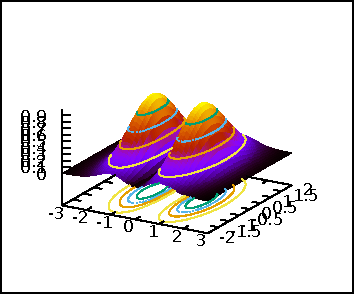
\includegraphics[width=.5\textwidth]{wxdraw3d_h.pdf}
 \hfill
\end{maximat}

\section{Límites}

En Maxima no existe ninguna función para calcular límites
de funciones en varias variables de manera directa.
Así que tendremos que buscar otros métodos para estudiarlos.

\subsection{Límites iterados}

Una forma de comprobar la posible existencia de un límite
en dos variables es calculando los límites iterados,
existen dos límites iterados que son
\begin{equation*}
 \lim_{x\to x_0}\lim_{y\to y_0} f(x,y)
 \quad\text{ y }\quad
 \lim_{y\to y_0}\lim_{x\to x_0} f(x,y),
\end{equation*}
Para ello nos basamos en el comando \maximain{limit} que
calcula límites en una variable, los límites anteriores
se pueden calcular, respectivamente, en Maxima con
\begin{center}
 \maximain{limit(limit(f(x,y),y,y0),x,x0)}
 \quad y \quad
 \maximain{limit(limit(f(x,y),x,x0),y,y0)}
\end{center}
Por ejemplos los límites iterados
en el punto $(0,0)$ de la función $g$
definida previamente son los siguientes.
\begin{maximai}
 limit(limit(g(x,y),y,0),x,0)
\end{maximai}
\begin{maximao}
 0
\end{maximao}
\begin{maximai}
 limit(limit(g(x,y),x,0),y,0);
\end{maximai}
\begin{maximao}
 0
\end{maximao}
En este caso, no podemos asegurar que el límite
\begin{equation*}
 \lim_{(x,y)\to (0,0)} g(x,y);
\end{equation*}
sea $0$, pero si existiese la única posibilidad
es que su valor sea $0$.

Si ahora queremos estudiar el límite
\begin{equation*}
 \lim_{(x,y)\to (0,0)} \frac{x^2-y}{x^5+y}
\end{equation*}
con límites iterados, haríamos lo siguiente.
\begin{maximai}
 limit(limit((x^2-y)/(x^5+y),y,0),x,0);
\end{maximai}
\begin{maximao}
 \ensuremath{\mathrm{infinity}}
\end{maximao}
\begin{maximai}
 limit(limit((x^2-y)/(x^5+y),x,0),y,0);
\end{maximai}
\begin{maximao}
 -1
\end{maximao}
En este caso, ya que los límites iterados son distintos
podemos asegurar que el límite no existe.

%\subsection{Límites en coordenadas polares}

\subsection{Límites en una dirección}

Cuando se calculan los límites iterados, se está obteniendo
la información del límite cuando nos acercamos en las direcciones
de los ejes.
Sin embargo, hay ocasiones que los límites iterados coinciden
aunque el límite no exista, en estos casos se puede recurrir
al estudio de los límites en una dirección diferente a los ejes.
Veamos un ejemplo donde ocurre esta situación,
considera la función $f(x,y) = \frac{xy^2}{x^3+y^3}$ y el límite
\begin{equation*}
 \lim_{(x,y)\to(0,0)} f(x,y).
\end{equation*}
Si se calculan los límites iterados el resultado de ambos será $0$.
Pero si se calcula el límite en la dirección del vector $v=(1,1)$
se puede ver que es diferente. El cálculo de este límite se hace con
la expresión
\begin{equation*}
 \lim_{t\to0} f(0 + t v_1, 0 + t v_2),
\end{equation*}
el cual se puede calcular en Maxima como
\begin{maximai}
 f(x,y):=x*y^2/(x^3+y^3)$
\end{maximai}\begin{maximal}
 v:[1,1]$
\end{maximal}\begin{maximal}
 limit(f(0+t*v[1],0+t*v[2]), t, 0);
\end{maximal}
\begin{maximao}
 \frac{1}{2}
\end{maximao}


\section{Diferenciabilidad}

\subsection{Derivadas parciales}
Para calcular derivadas parciales de una función $f$
usamos el comando \maximain{diff} usando como segundo
argumento la variable respecto a la cual se deriva.
De esa manera, para calcular
$\frac{\partial f}{\partial x}$
y
$\frac{\partial f}{\partial y}$
se hace
\begin{center}
 \maximain{diff(f(x,y),x)}
 \quad y \quad
 \maximain{diff(f(x,y),y)},
\end{center}
para calcular las derivadas cruzadas
$\frac{\partial^2 f}{\partial y\partial x}$
y
$\frac{\partial^2 f}{\partial x\partial y}$
se puede realizar, respectivamente, como
\begin{center}
 \maximain{diff(diff(f(x,y),x),y)}
 \quad y \quad
 \maximain{diff(diff(f(x,y),y),x)},
\end{center}
por último, para calcular
$\frac{\partial^2 f}{\partial x^2}$
y
$\frac{\partial^2 f}{\partial y^2}$
se hará respectivamente como
\begin{center}
 \maximain{diff(f(x,y),x,2)}
 \quad y \quad
 \maximain{diff(f(x,y),y,2)}.
\end{center}

Apliquemos lo anterior a un ejemplo,
calculemos las derivadas parciales de la función
$f(x,y) = x^2-3xy+5xy^3$.
\begin{maximai}
 f(x,y):=x^2-3*x*y+5*x*y^3$
\end{maximai}\begin{maximal}
 fx:diff(f(x,y),x);
\end{maximal}
\begin{maximao}
 5 {{y}^{3}}-3 y+2 x
\end{maximao}
\begin{maximai}
 fy:diff(f(x,y),y);
\end{maximai}
\begin{maximao}
 15 x {{y}^{2}}-3 x
\end{maximao}
\begin{maximai}
 fxy:diff(fx,y);
\end{maximai}
\begin{maximao}
 15 {{y}^{2}}-3
\end{maximao}
\begin{maximai}
 fyx:diff(fy,x);
\end{maximai}
\begin{maximao}
 15 {{y}^{2}}-3
\end{maximao}
\begin{maximai}
 fxx:diff(fx,x);
\end{maximai}
\begin{maximao}
 2
\end{maximao}
\begin{maximai}
 fyy:diff(fy,y);
\end{maximai}
\begin{maximao}
 30 x y
\end{maximao}
Si se quiere evaluar una derivada parcial en algún punto,
se podrá hacer de dos maneras, por ejemplo se muestra la
forma de calcular
\begin{equation*}
\frac{\partial^2 f}{\partial y^2}(-1,2).
\end{equation*}
\begin{maximai}
 ev(fyy, x=-1, y=2);
\end{maximai}
\begin{maximao}
 -60
\end{maximao}
\begin{maximai}
 fyy, x=-1, y=2;
\end{maximai}
\begin{maximao}
 -60
\end{maximao}

\subsection{Derivadas direccionales}

Dado un vector
$u = (u_1, u_2)$,
se define la derivada direccional
de una función $f$ en un punto $(x_0, y_0)$
como
\begin{equation*}
 D_uf(x_0,y_0) =
 \lim_{t\to0} \frac{f(x_0+tu_1,y_0+tu_2)-f(x_0,y_0)}{t},
\end{equation*}
cuyo valor se puede calcular
usando las derivadas parciales con la expresión
\begin{equation*}
 D_uf(x_0,y_0) =
 \frac{\partial f}{\partial x}(x_0,y_0)u_1
 +
 \frac{\partial f}{\partial y}(x_0,y_0)u_2.
\end{equation*}
A continuación se realiza un ejemplo en Maxima
calculando $D_uf(x_0,y_0)$ siendo la función
$f$ definida anteriormente,
$u=(1,1)$
y $(x_0,y_0) = (-1,2)$.
\begin{maximai}
 x0:-1$ y0:2$
\end{maximai}
\begin{maximai}
 u:[1,1];
\end{maximai}
\begin{maximao}
 \left[ 1\operatorname{,}1\right]
\end{maximao}
\begin{maximai}
 limit((f(x0+t*u[1],y0+t*u[2]) - f(x0,y0))/t, t, 0);
\end{maximai}
\begin{maximao}
 -25
\end{maximao}
\begin{maximai}
 ev(fx*u[1]+fy*u[2], x=x0, y=y0);
\end{maximai}
\begin{maximao}
 -25
\end{maximao}


\section{Gradiente}

Dada una función de dos variables $f$ se define
el vector gradiente como
\begin{equation*}
 \nabla f =
 \left(
 \frac{\partial f}{\partial x},
 \frac{\partial f}{\partial y}
 \right).
\end{equation*}
Por tanto se puede calcular en Maxima como mostramos
para la función $f$ definida anteriormente.
\begin{maximai}
 gradf:[diff(f(x,y),x), diff(f(x,y),y)];
\end{maximai}
\begin{maximao}
 \left[ 5 {{y}^{3}}-3 y+2 x\operatorname{,}15 x {{y}^{2}}-3 x\right]
\end{maximao}
O si ya se tiene definido las derivadas parciales
se podría calcular como sigue.
\begin{maximai}
 gradf:[fx, fy];
\end{maximai}
\begin{maximao}
 \left[ 5 {{y}^{3}}-3 y+2 x\operatorname{,}15 x {{y}^{2}}-3 x\right]
\end{maximao}

\section{Divergencia y rotacional}
Recordemos que para una función vectorial de tres variables
$g(x,y,z) = (g_1(x,y,z), g_2(x,y,z), g_3(x,y,z))$
se define la divergencia como
\begin{equation*}
 \divop g =
 \frac{\partial g_1}{\partial x}
 +\frac{\partial g_2}{\partial y}
 +\frac{\partial g_3}{\partial z},
\end{equation*}
y el rotacional como
\begin{equation*}
 \rotop g =
 \left(
 \frac{\partial g_3}{\partial y}
 -\frac{\partial g_2}{\partial z},
 \frac{\partial g_1}{\partial z}
 -\frac{\partial g_3}{\partial x},
 \frac{\partial g_2}{\partial x}
 -\frac{\partial g_1}{\partial y}
 \right).
\end{equation*}
Por tanto para calcular la divergencia y el rotacional
a la función
$g(x,y,z) = (2xy, y^2z, xyz^2)$
se haría lo siguiente.
\begin{maximai}
 g(x,y,z):=[2*x*y,y^2*z,x*y*z^2]$
\end{maximai}
\begin{maximai}
 diver:diff(g(x,y,z)[1],x) + diff(g(x,y,z)[2],y) + diff(g(x,y,z)[3],z);
\end{maximai}
\begin{maximao}
 2 x y z+2 y z+2 y
\end{maximao}
\begin{maximai}
 rot:[
\end{maximai} \begin{maximal}
  diff(g(x,y,z)[3],y) - diff(g(x,y,z)[2],z),
\end{maximal} \begin{maximal}
  diff(g(x,y,z)[1],z) - diff(g(x,y,z)[3],x),
\end{maximal} \begin{maximal}
  diff(g(x,y,z)[2],x) - diff(g(x,y,z)[1],y)
\end{maximal} \begin{maximal}
 ];
\end{maximal}
\begin{maximao}
 \left[
  x {{z}^{2}}-{{y}^{2}}\operatorname{,}
  -y {{z}^{2}}\operatorname{,}
  -2 x
  \right]
\end{maximao}
